\documentclass[aspectratio=169,10pt]{beamer}

\usetheme{Madrid}
\usecolortheme{seahorse}

\usepackage{amsmath}
\usepackage{amssymb}
\usepackage{amsfonts}
\usepackage{mathtools}
\usepackage{listings}
\usepackage{xcolor}
\usepackage{graphicx}
\usepackage{multicol}
\usepackage{hyperref}

% Configure graphics path
\graphicspath{{figures/}}

% Configure listings for code
\lstset{
    basicstyle=\ttfamily\scriptsize,
    commentstyle=\color{green!50!black}\itshape,
    keywordstyle=\color{blue}\bfseries,
    stringstyle=\color{red},
    breaklines=true,
    breakatwhitespace=true,
    numbers=left,
    numberstyle=\tiny\color{gray},
    frame=single,
    framexleftmargin=5pt,
    language=Python,
    showstringspaces=false,
}

% Customization
\setbeamertemplate{footline}[frame number]
\setbeamercovered{transparent}

% Title slide
\title[Sums of Monotone Operators]{Chapter 25: Sums of Monotone Operators \\ Infimal Postcomposition and Composition Operations}
\author{Convex Analysis and Monotone Operator Theory}
\institute{Based on Bauschke \& Combettes (2017)}
\date{}

\begin{document}

% Title Slide
\frame{\titlepage}

% Table of Contents
\begin{frame}
  \frametitle{Table of Contents}
  \tableofcontents[hideallsubsections]
\end{frame}

\section{Introduction and Motivation}

\begin{frame}
  \frametitle{Overview of Chapter 25}

  This chapter explores the properties of sums of monotone operators and their compositions:

  \begin{itemize}
    \item \textbf{Maximal Monotonicity of Sums}: When is $A + B$ maximally monotone?
    \item \textbf{Local Properties}: Local maximal monotonicity versus global properties
    \item \textbf{3* Monotone Operators}: Special class of monotone operators (Brézis-Haraux)
    \item \textbf{Sum Theorems}: Conditions ensuring sum is maximally monotone
    \item \textbf{Parallel Operations}: Parallel sum and parallel composition
    \item \textbf{Infimal Postcomposition}: Extension of infimal convolution to operators
  \end{itemize}

  \vspace{0.3cm}

  \textbf{Key Result}: Under appropriate conditions, the sum $A + B$ of two monotone operators is maximally monotone.

\end{frame}

\begin{frame}
  \frametitle{Motivation: Why Study Sums?}

  \begin{columns}
    \column{0.48\textwidth}
    \textbf{Problem Decomposition}
    \begin{itemize}
      \item Many optimization problems involve sums: $\min_x f(x) + g(x)$
      \item Corresponds to monotone operators: $\partial f + \partial g$
      \item Want to solve using splitting methods
    \end{itemize}

    \vspace{0.3cm}

    \textbf{Applications}
    \begin{itemize}
      \item Proximal algorithms
      \item Operator splitting
      \item Composite optimization
      \item Duality theory
    \end{itemize}

    \column{0.48\textwidth}
    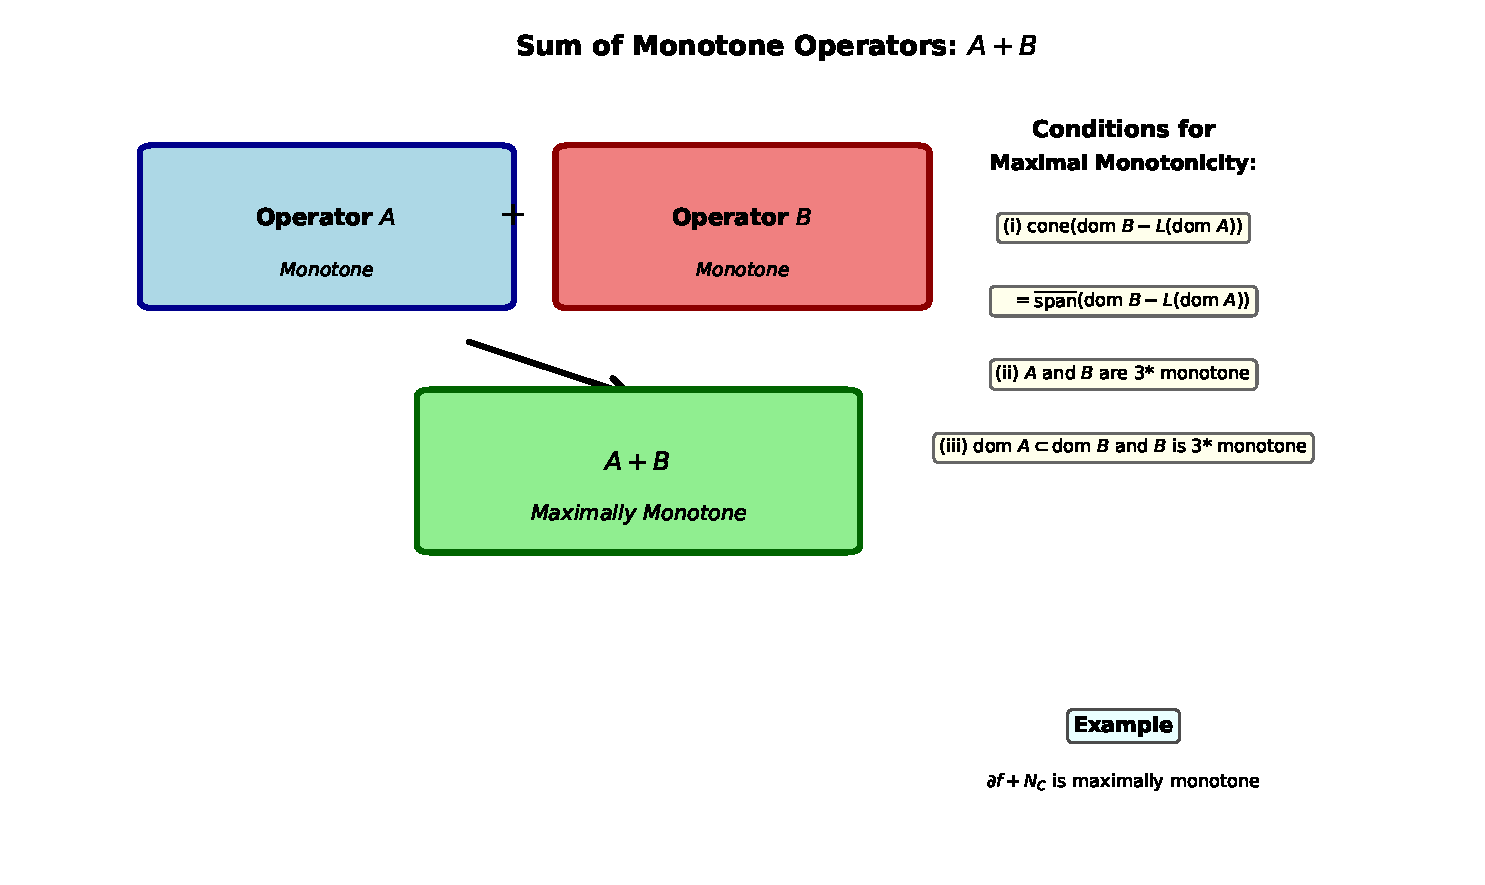
\includegraphics[width=\textwidth]{monotone_sum}
  \end{columns}

\end{frame}

\section{Maximal Monotonicity of Sums and Composite Sums}

\begin{frame}
  \frametitle{Canonical Sum and Elementary Properties}

  \textbf{Proposition 25.1 (Canonical Sum)}

  Let $A, B: \mathcal{H} \to 2^{\mathcal{H}}$ be monotone operators. For every $x \in \mathcal{H}$:
  $$A(x) + B(x) = \{u + v : u \in A(x), \, v \in B(x)\}$$

  \vspace{0.3cm}

  \textbf{Proposition 25.2 (Composite Operators)}

  Let $A, B: \mathcal{H} \to 2^{\mathcal{H}}$ be monotone. Then:
  \begin{align*}
    &\text{dom}(A + B) = \text{dom} A \cap \text{dom} B \\
    &\text{ran}(A + B) = \text{ran} A + \text{ran} B \\
    &\text{gra}(A + B) = \text{gra} A + \text{gra} B
  \end{align*}

\end{frame}

\begin{frame}
  \frametitle{Sufficient Conditions for Maximal Monotonicity}

  \textbf{Theorem 25.3 (Sufficient Condition via Cone)}

  Let $A: \mathcal{H} \to 2^{\mathcal{H}}$ and $B: \mathcal{K} \to 2^{\mathcal{K}}$ be maximally monotone,
  $L \in \mathcal{B}(\mathcal{H}, \mathcal{K})$, and suppose:
  $$\text{cone}(\text{dom } B - L(\text{dom } A)) = \overline{\text{span}}(\text{dom } B - L(\text{dom } A))$$

  Then $A + L^* B L$ is maximally monotone.

  \vspace{0.3cm}

  \textbf{Example 25.3}
  $$\text{If } L \in \mathcal{B}(\mathcal{H}, \mathcal{K}), \, A: \mathcal{H} \to 2^{\mathcal{H}}, \, B = N_{\text{gra } L}$$
  then $A + L^* BL$ is maximally monotone.

\end{frame}

\begin{frame}
  \frametitle{Key Sufficient Conditions}

  \textbf{Corollary 25.5}

  Let $A, B: \mathcal{H} \to 2^{\mathcal{H}}$ be maximally monotone. If any one of:

  \begin{enumerate}
    \item[(i)] $\text{dom } B = \mathcal{H}$
    \item[(ii)] $\text{dom } A \cap \text{int } \text{dom } B \neq \emptyset$
    \item[(iii)] $0 \in \text{int}(\text{dom } A - \text{dom } B)$
    \item[(iv)] $(\forall x \in \mathcal{H})(\exists \varepsilon \in \mathbb{R}_{++}) \, [0, \varepsilon x] \subset \text{dom } A - \text{dom } B$
    \item[(v)] $\text{dom } A$ and $\text{dom } B$ convex, $0 \in \text{sri}(\text{dom } A - \text{dom } B)$
  \end{enumerate}

  \textbf{Then } $A + B$ is maximally monotone.

\end{frame}

\section{Local Maximal Monotonicity}

\begin{frame}
  \frametitle{Definition and Motivation}

  \textbf{Definition 25.7 (Locally Maximally Monotone)}

  Let $A: \mathcal{H} \to 2^{\mathcal{H}}$ be monotone and $U$ an open convex subset of $\mathcal{H}$ such that $U \cap \text{ran } A \neq \emptyset$.

  $A$ is \textbf{locally maximally monotone with respect to $U$} if: for every $(x, u) \in (\mathcal{H} \times U) \setminus \text{gra } A$,
  there exists $(y, v) \in (\mathcal{H} \times U) \cap \text{gra } A$ such that
  $$\langle x - y \mid u - v \rangle < 0$$

  \vspace{0.3cm}

  \textbf{Definition (Globally Locally Maximally Monotone)}

  $A$ is \textbf{locally maximally monotone} if it is locally maximally monotone with respect to every open convex subset of $\mathcal{H}$ with nonempty intersection with $\text{ran } A$.

\end{frame}

\begin{frame}
  \frametitle{Relationship to Maximal Monotonicity}

  \textbf{Proposition 25.8}

  Let $A: \mathcal{H} \to 2^{\mathcal{H}}$ be monotone. Then:

  \begin{enumerate}
    \item[(i)] $A$ is locally maximally monotone with respect to $\mathcal{H}$ if and only if $A$ is maximally monotone.
    \item[(ii)] $A$ is locally maximally monotone if and only if, for every bounded closed convex subset $C$ of $\mathcal{H}$
      such that $\text{ran } A \cap \text{int } C \neq \emptyset$ and for every $(x, u) \in (\mathcal{H} \times \text{int } C) \setminus \text{gra } A$,
      there exists $(y, v) \in (\mathcal{H} \times C) \cap \text{gra } A$ such that $\langle x - y \mid u - v \rangle < 0$.
  \end{enumerate}

  \vspace{0.3cm}

  \textbf{Proposition 25.9}

  If $A: \mathcal{H} \to 2^{\mathcal{H}}$ is maximally monotone, then $A$ is locally maximally monotone.

\end{frame}

\section{3* Monotone Operators (Brézis-Haraux)}

\begin{frame}
  \frametitle{Definition of 3* Monotone Operators}

  \textbf{Definition 25.10 (3* Monotone)}

  Let $A: \mathcal{H} \to 2^{\mathcal{H}}$ be monotone. Then $A$ is \textbf{3* monotone} if:
  $$\text{dom } A \times \text{ran } A \subset \text{dom } F_A$$

  where $F_A(x, y) = \sup_{(z,w) \in \text{gra } A} (\langle x - z \mid w \rangle + \langle z - y \mid w \rangle)$.

  \vspace{0.3cm}

  \textbf{Interpretation}: The graph of $A$ has a special rectangular structure in the product space.

\end{frame}

\begin{frame}
  \frametitle{Characterizations of 3* Monotone Operators}

  \textbf{Proposition 25.11}

  Let $A: \mathcal{H} \to 2^{\mathcal{H}}$ be maximally monotone and 3* monotone. Then:
  $$\text{dom } F_A = \text{dom } A \times \overline{\text{ran}} A$$

  \vspace{0.3cm}

  \textbf{Proposition 25.12}

  If $A$ is 3-cyclically monotone, then $A$ is 3* monotone.

  \vspace{0.3cm}

  \textbf{Examples 25.13 \& 25.14}

  \begin{itemize}
    \item If $f: \mathcal{H} \to [-\infty, +\infty]$ is proper, then $\partial f$ is 3* monotone.
    \item If $C$ is a nonempty closed convex subset of $\mathcal{H}$, then $N_C$ is 3* monotone.
  \end{itemize}

\end{frame}

\begin{frame}[fragile]
  \frametitle{3* Monotone: Characterization (Proposition 25.16)}

  \textbf{Proposition 25.16}

  Let $A \in \mathcal{B}(\mathcal{H})$ be monotone. The following are equivalent for some $\beta \in \mathbb{R}_{++}$:

  \begin{enumerate}
    \item[(i)] $A$ is 3* monotone.
    \item[(ii)] $A$ is $\beta$-cocoercive.
    \item[(iii)] $A^*$ is $\beta$-cocoercive.
    \item[(iv)] $A^*$ is 3* monotone.
  \end{enumerate}

  \vspace{0.3cm}

  \textbf{Python Example: Detecting 3* Monotone Operators}

  \begin{lstlisting}
# For a matrix A (operator in finite dimensions)
# Check if A is beta-cocoercive (hence 3* monotone)
import numpy as np

def is_cocoercive(A, beta):
    """Check if operator A is beta-cocoercive"""
    eigenvalues = np.linalg.eigvals(A + A.T) / 2
    min_eigenval = np.min(eigenvalues)
    return min_eigenval >= beta
  \end{lstlisting}

\end{frame}

\section{The Brézis-Haraux Theorem}

\begin{frame}
  \frametitle{Theorem 25.23 (Simons)}

  \textbf{Theorem 25.23 (Simons)}

  Let $A, B: \mathcal{H} \to 2^{\mathcal{H}}$ be monotone operators such that $A + B$ is maximally monotone. Suppose that:
  $$(\forall u \in \text{ran } A)(\forall v \in \text{ran } B)(\exists x \in \mathcal{H}) \quad (x, u) \in \text{dom } F_A \text{ and } (x, v) \in \text{dom } F_B$$

  Then:
  $$\overline{\text{ran } A + \text{ran } B} = \overline{\text{ran}(A + B)} \quad \text{and} \quad \text{int} \text{ran}(A + B) = \text{int}(\text{ran } A + \text{ran } B)$$

  \vspace{0.3cm}

  This characterizes the range of the sum in terms of the sum of ranges.

\end{frame}

\begin{frame}
  \frametitle{Theorem 25.24 (Brézis-Haraux)}

  \textbf{Theorem 25.24 (Brézis-Haraux)}

  Let $A, B: \mathcal{H} \to 2^{\mathcal{H}}$ be monotone operators such that $A + B$ is maximally monotone.

  If one of the following conditions holds:

  \begin{enumerate}
    \item[(i)] $A$ and $B$ are 3* monotone.
    \item[(ii)] $\text{dom } A \subset \text{dom } B$ and $B$ is 3* monotone.
  \end{enumerate}

  Then:
  $$\overline{\text{ran}(A + B)} = \overline{\text{ran } A + \text{ran } B} \quad \text{and} \quad \text{int } \text{ran}(A + B) = \text{int}(\text{ran } A + \text{ran } B)$$

\end{frame}

\begin{frame}
  \frametitle{Applications of Brézis-Haraux}

  \textbf{Corollary 25.27}

  Let $A, B: \mathcal{H} \to 2^{\mathcal{H}}$ be monotone operators such that $A + B$ is maximally monotone, $A$ or $B$ is surjective, and one of:

  \begin{enumerate}
    \item[(i)] $A$ and $B$ are 3* monotone.
    \item[(ii)] $\text{dom } A \subset \text{dom } B$ and $B$ is 3* monotone.
  \end{enumerate}

  Then $A + B$ is surjective (i.e., $A + B$ is in one-to-one correspondence).

  \vspace{0.3cm}

  \textbf{Example 25.25}: If $C$ and $D$ are closed convex cones, then $N_C + N_D = \mathbb{R} \times \{0\}$ fails unless both are maximally monotone, showing necessity of assumptions.

\end{frame}

\section{Parallel Sum}

\begin{frame}
  \frametitle{Parallel Sum Operation}

  \textbf{Definition 25.29 (Parallel Sum)}

  Let $A, B: \mathcal{H} \to 2^{\mathcal{H}}$ be operators. The \textbf{parallel sum} of $A$ and $B$ is:
  $$A \square B = (A^{-1} + B^{-1})^{-1}$$

  \vspace{0.3cm}

  \textbf{Motivation}: In network/circuit theory, parallel combination of impedances/conductances.

  \vspace{0.3cm}

  \textbf{Connection to Infimal Convolution}:
  For functions $f, g: \mathcal{H} \to [-\infty, +\infty]$:
  $$(f \square g) = (\partial f) \square (\partial g)$$

\end{frame}

\begin{frame}
  \frametitle{Properties of Parallel Sum}

  \textbf{Proposition 25.30}

  Let $A, B: \mathcal{H} \to 2^{\mathcal{H}}$ be operators, and let $x, u \in \mathcal{H}$. Then:

  \begin{enumerate}
    \item[(i)] $(A \square B)x = \bigcup_{y \in \mathcal{H}} (A(y) \cap B(x - y))$
    \item[(ii)] $u \in (A \square B)x \Leftrightarrow (\exists y \in \mathcal{H}) \, y \in A^{-1}u \text{ and } x - y \in B^{-1}u$
    \item[(iii)] $\text{dom}(A \square B) = \text{ran}(A^{-1} + B^{-1})$
    \item[(iv)] $\text{ran}(A \square B) = \text{ran} A \cap \text{ran} B$
    \item[(v)] If $A, B$ are monotone, then $A \square B$ is monotone.
  \end{enumerate}

\end{frame}

\begin{frame}
  \frametitle{Parallel Sum for Convex Functions}

  \textbf{Proposition 25.32}

  Let $f, g \in \Gamma_0(\mathcal{H})$ and suppose $0 \in \text{sri}(\text{dom } f^* - \text{dom } g^*)$. Then:
  $$(\partial f) \square (\partial g) = \partial(f \square g)$$

  where the parallel sum of functions is:
  $$(f \square g)(x) := \inf_{y \in \mathcal{H}} f(y) + g(x - y)$$

  \vspace{0.3cm}

  \textbf{Properties}:
  \begin{itemize}
    \item $f \square g \in \Gamma_0(\mathcal{H})$
    \item $\text{dom}(f \square g) = \text{dom} f + \text{dom} g$
  \end{itemize}

\end{frame}

\begin{frame}[fragile]
  \frametitle{Numerical Example: Parallel Sum}

  \textbf{Example}: Quadratic functions and their parallel sum

  \begin{lstlisting}
import numpy as np

# Define quadratic functions f(x) = (1/2)||x||^2
# and g(x) = (1/2)||x - c||^2

def parallel_sum_quadratic(x, c, lambda_f=1.0, lambda_g=1.0):
    """Parallel sum of two quadratic functions"""
    # For quadratics: (f square g)(x) is also quadratic
    # Parameters combine harmonically
    lambda_sum = 1 / (1/lambda_f + 1/lambda_g)
    center = lambda_sum * c / lambda_g
    return 0.5 * lambda_sum * (np.linalg.norm(x - center) ** 2)

# Example with c = [1, 0]
x = np.array([0.5, 0.5])
c = np.array([1.0, 0.0])
result = parallel_sum_quadratic(x, c)
print(f"Parallel sum at x: {result}")
  \end{lstlisting}

\end{frame}

\section{Parallel Composition and Infimal Postcomposition}

\begin{frame}
  \frametitle{Parallel Composition Definition}

  \textbf{Definition 25.39 (Parallel Composition)}

  Let $\mathcal{K}$ be a real Hilbert space, $A: \mathcal{H} \to 2^{\mathcal{H}}$, and $L \in \mathcal{B}(\mathcal{H}, \mathcal{K})$.
  The \textbf{parallel composition} of $A$ by $L$ is the operator from $\mathcal{K}$ to $2^{\mathcal{K}}$:
  $$L \triangledown A = (L \circ A^{-1} \circ L^*)^{-1}$$

  \vspace{0.3cm}

  \textbf{Alternative names}:
  \begin{itemize}
    \item Infimal postcomposition
    \item Pushforward with infimal convolution
  \end{itemize}

  \vspace{0.3cm}

  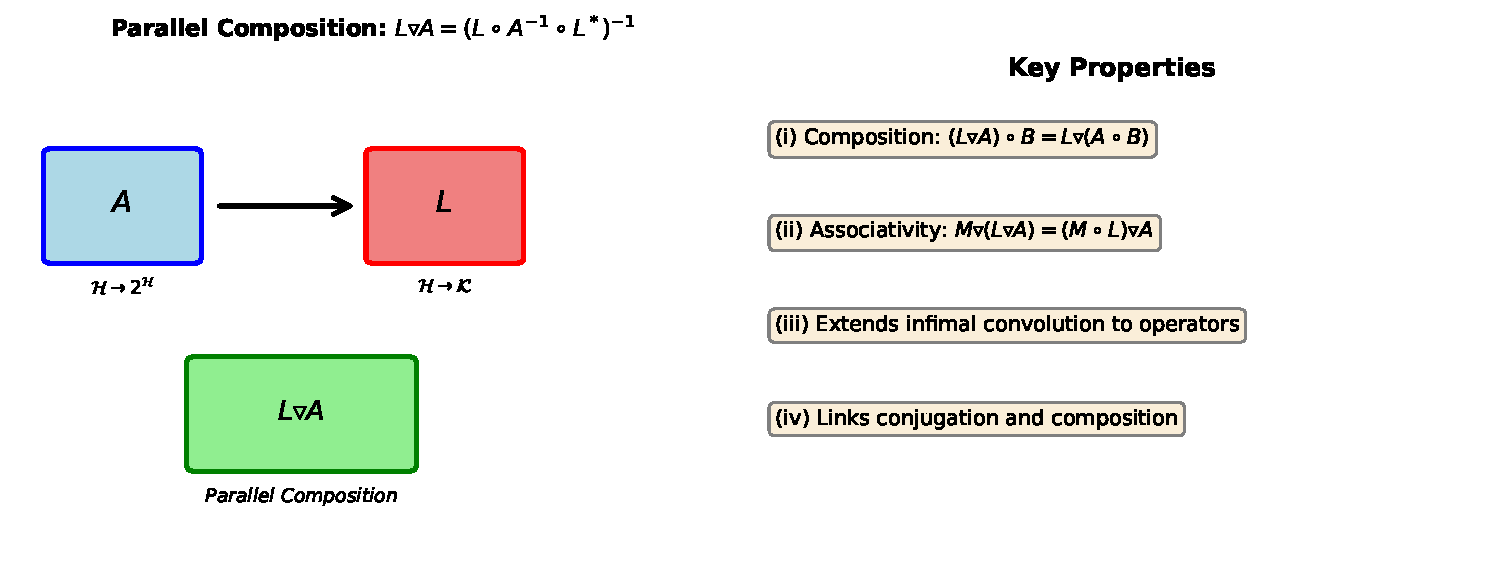
\includegraphics[width=0.8\textwidth]{parallel_composition}

\end{frame}

\begin{frame}
  \frametitle{Parallel Composition Properties}

  \textbf{Proposition 25.41}

  Let $\mathcal{K}$ be a real Hilbert space, $A: \mathcal{H} \to 2^{\mathcal{H}}$, $B: \mathcal{K} \to 2^{\mathcal{K}}$ be monotone,
  $L \in \mathcal{B}(\mathcal{H}, \mathcal{K})$. Then:

  \begin{enumerate}
    \item[(i)] $(L \triangledown A) \square B)^{-1} = L \circ A^{-1} \circ L^* + B^{-1}$
    \item[(ii)] If $A, B$ monotone, then $(L \triangledown A) \square B$ is monotone.
    \item[(iii)] If $A, B$ maximally monotone and $\text{cone}(\text{ran } A - L^*(\text{ran } B)) = \text{span}(\text{ran } A - L^*(\text{ran } B))$,
      then $(L \triangledown A) \square B$ is maximally monotone.
  \end{enumerate}

\end{frame}

\begin{frame}
  \frametitle{Connection to Function Composition}

  \textbf{Proposition 25.42}

  Let $G, \mathcal{K}$ be real Hilbert spaces, $A: \mathcal{H} \to 2^{\mathcal{H}}$, $B: \mathcal{H} \to 2^{\mathcal{H}}$,
  $L \in \mathcal{B}(\mathcal{G}, \mathcal{H})$, $M \in \mathcal{B}(\mathcal{G}, \mathcal{K})$. Then:

  \begin{enumerate}
    \item[(i)] $L \triangledown (A \square B) = (L \triangledown A) \square (L \triangledown B)$
    \item[(ii)] $M \triangledown (L \triangledown A) = (M \circ L) \triangledown A$
  \end{enumerate}

  \vspace{0.3cm}

  These are the main composition properties for parallel composition of operators.

\end{frame}

\begin{frame}
  \frametitle{Infimal Postcomposition for Convex Functions}

  \textbf{Proposition 25.43}

  Let $\mathcal{K}$ be a real Hilbert space, $f \in \Gamma_0(\mathcal{H})$, $g \in \Gamma_0(\mathcal{K})$,
  $L \in \mathcal{B}(\mathcal{H}, \mathcal{K})$ such that $0 \in \text{sri}(\text{dom } f^* - L^*(\text{dom } g^*))$. Then:

  \begin{enumerate}
    \item[(i)] $L \triangledown f \in \Gamma_0(\mathcal{K})$
    \item[(ii)] $\partial(L \triangledown f) \square g = (L \triangledown \partial f) \square g$
  \end{enumerate}

  \vspace{0.3cm}

  This links infimal postcomposition for functions to that for operators.

\end{frame}

\begin{frame}[fragile]
  \frametitle{Operator Hierarchy and Examples}

  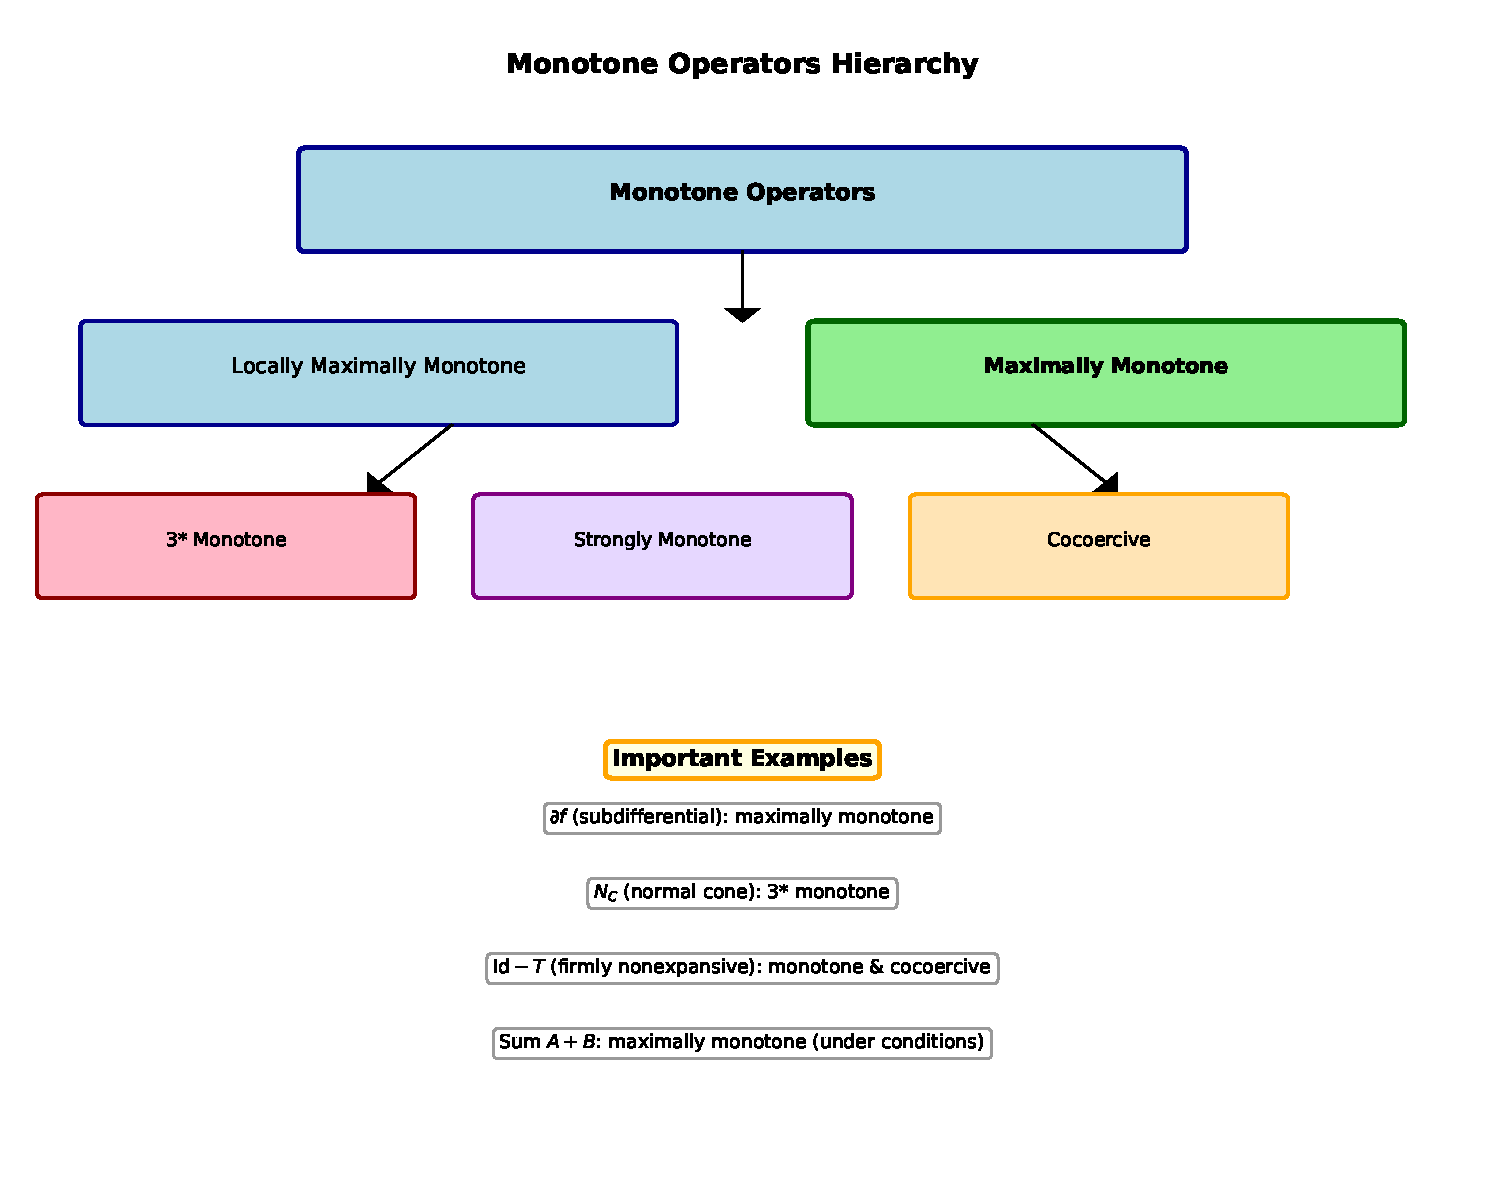
\includegraphics[width=\textwidth]{operator_hierarchy}

\end{frame}

\begin{frame}[fragile]
  \frametitle{Key Examples of 3* Monotone Operators}

  \textbf{Example 25.15}: Conditions for 3* Monotonicity

  Let $A: \mathcal{H} \to 2^{\mathcal{H}}$ be monotone. Then $\text{dom } A \times \mathcal{H} \subset \text{dom } F_A$ and
  $A$ is 3* monotone in each case:

  \begin{enumerate}
    \item[(i)] $(\forall x \in \text{dom } A) \, \lim_{\rho \to +\infty} \inf_{\substack{(z,w) \in \text{gra } A \\ \|z\| \geq \rho}} \frac{\langle z - x \mid w \rangle}{\|z\|} = +\infty$
    \item[(ii)] $\text{dom } A$ is bounded.
    \item[(iii)] $A$ is uniformly monotone with a supercoercive modulus.
    \item[(iv)] $A$ is strongly monotone.
  \end{enumerate}

  \vspace{0.3cm}

  \textbf{Example 25.17}: $LL^*$ is 3* monotone.

\end{frame}

\section{Composite Operators and Extensions}

\begin{frame}
  \frametitle{Composite Operators: $(T \circ A)$ and $(A \circ T)$}

  \textbf{For $T: \mathcal{H} \to \mathcal{H}$ nonexpansive and $A: \mathcal{H} \to 2^{\mathcal{H}}$ monotone:}

  \begin{itemize}
    \item \textbf{Precomposition}: $T \circ A$ (operator before $A$)
    \item \textbf{Postcomposition}: $A \circ T$ (operator after $T$)
  \end{itemize}

  \vspace{0.3cm}

  \textbf{Example 25.18}: If $R$ is the cyclic right-shift operator, then $\text{Id} - R$ is 3* monotone.

  \vspace{0.3cm}

  \textbf{Example 25.20}:
  Let $D$ be nonempty, $T: D \to \mathcal{H}$, $A: \mathcal{H} \to 2^{\mathcal{H}}$ monotone, $\beta, \gamma \in \mathbb{R}_{++}$.

  If any one of (i)-(v) holds, then $T$ is 3* monotone:
  \begin{enumerate}
    \item[(i)] $T$ is $\beta$-cocoercive.
    \item[(ii)] $T$ is firmly nonexpansive.
    \item[(iii)] $T = J_{\gamma A}$ (resolvent).
    \item[(iv)] $T = \gamma A$ (scaled operator).
    \item[(v)] $\text{Id} - T$ is nonexpansive.
  \end{enumerate}

\end{frame}

\begin{frame}
  \frametitle{Proposition 25.19: Characterization of 3* Monotone Operators}

  \textbf{Proposition 25.19}

  Let $A: \mathcal{H} \to 2^{\mathcal{H}}$ be monotone and let $\gamma \in \mathbb{R}_{++}$. Then:

  \begin{enumerate}
    \item[(i)] $A$ is 3* monotone if and only if $A^{-1}$ is 3* monotone.
    \item[(ii)] $A$ is 3* monotone if and only if $\gamma A$ is 3* monotone.
  \end{enumerate}

  \vspace{0.3cm}

  This shows 3* monotonicity is preserved under inversion and scaling.

\end{frame}

\begin{frame}
  \frametitle{Composition Flow: From Functions to Operators}

  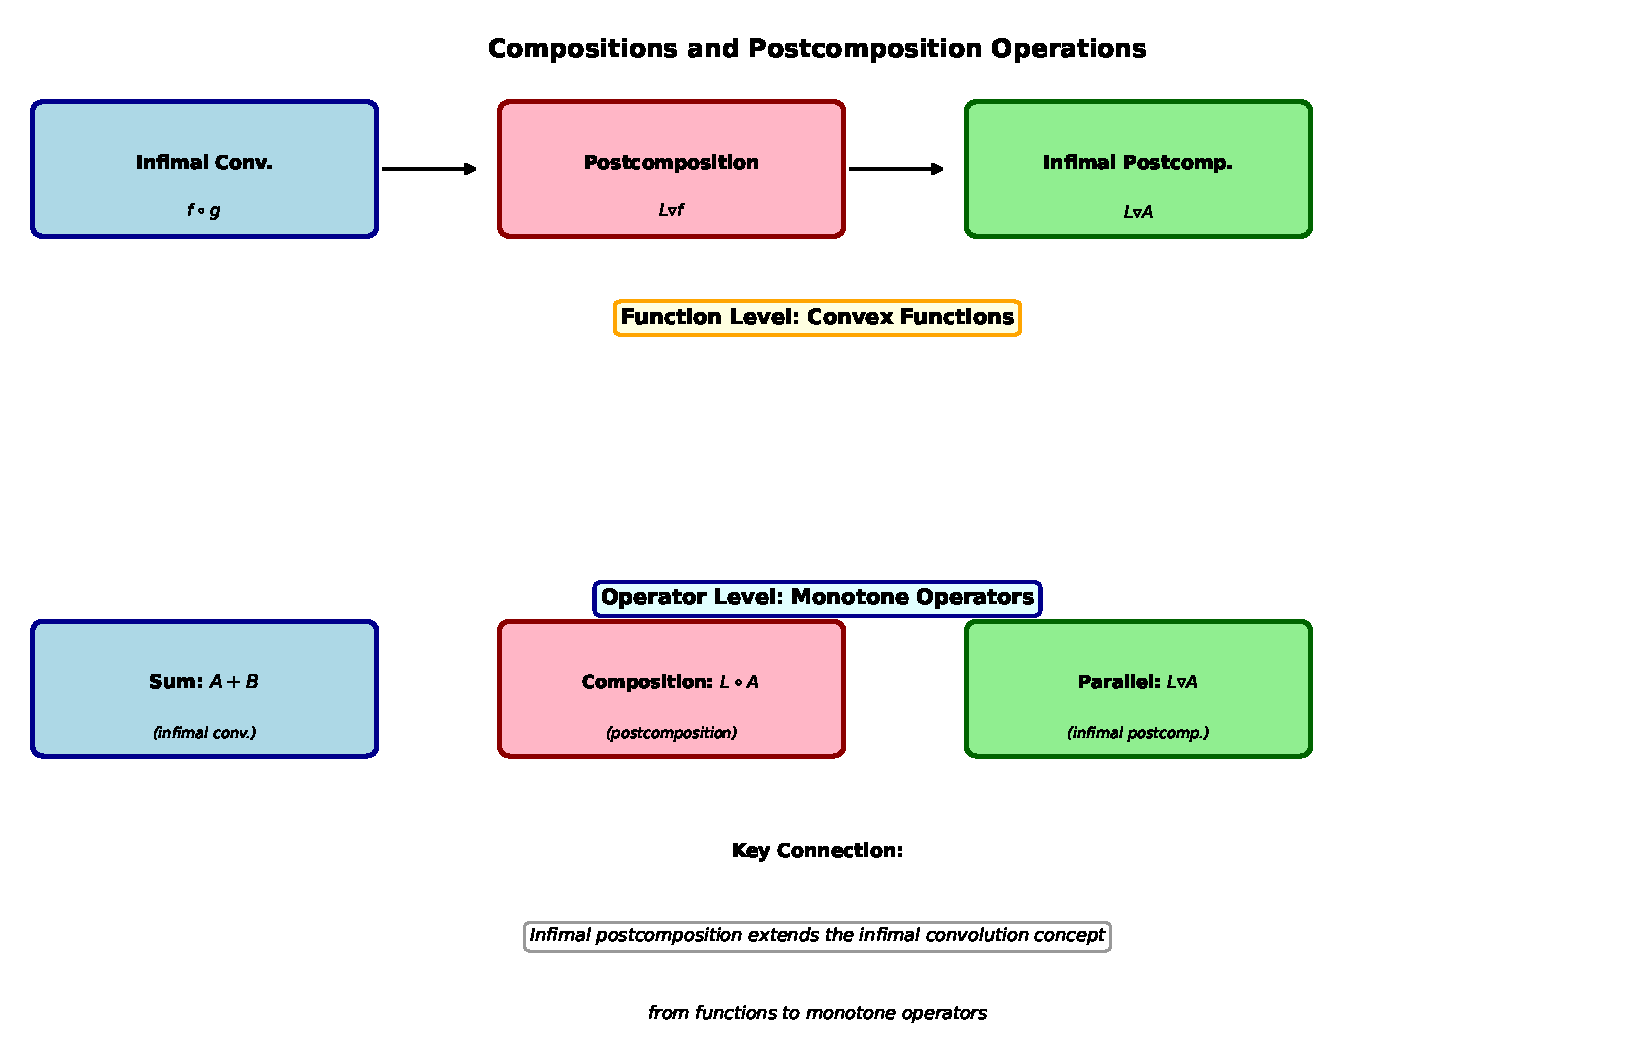
\includegraphics[width=\textwidth]{composition_flow}

\end{frame}

\section{Numerical and Computational Examples}

\begin{frame}[fragile]
  \frametitle{Numerical Examples}

  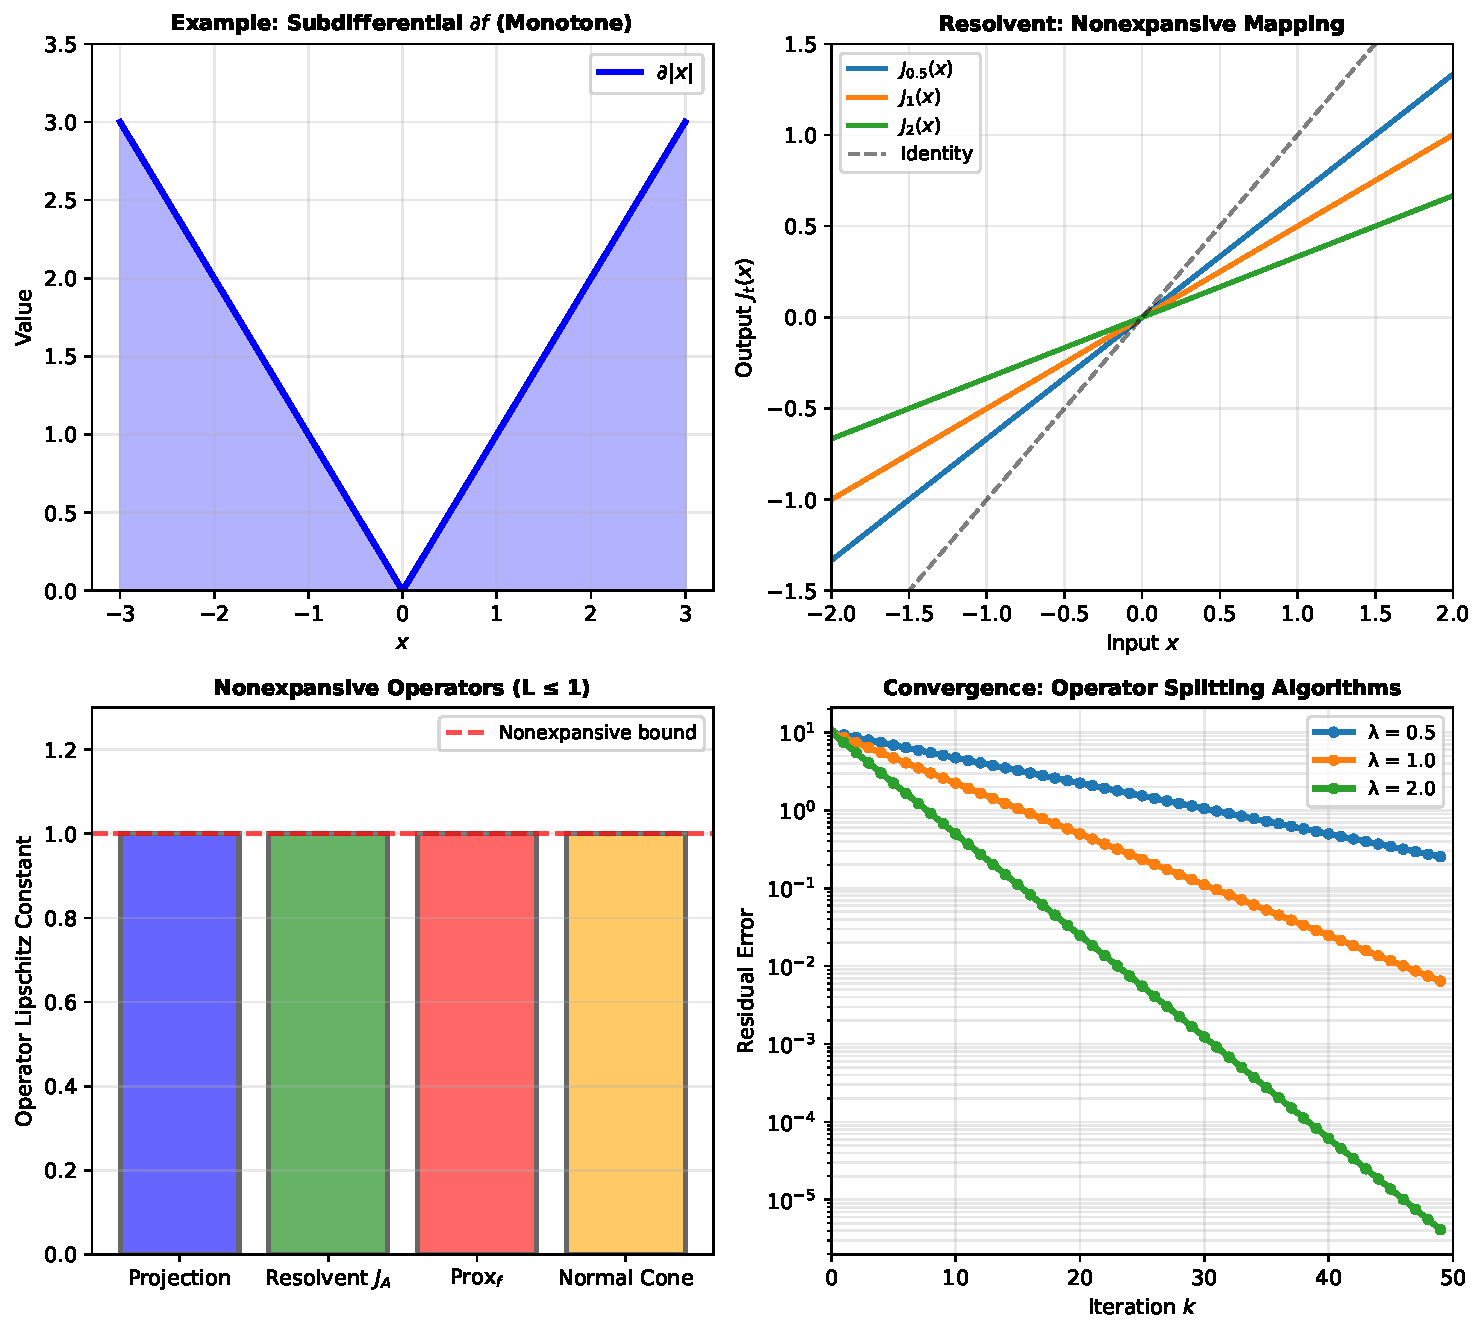
\includegraphics[width=\textwidth]{numerical_examples}

\end{frame}

\begin{frame}[fragile]
  \frametitle{Computing with Monotone Operators: Douglas-Rachford}

  \textbf{Problem}: Find $x \in \mathcal{H}$ such that $0 \in (A + B)x$ where $A, B$ maximally monotone.

  \vspace{0.2cm}

  \textbf{Douglas-Rachford Splitting}:

  \begin{lstlisting}
def douglas_rachford(A_inv, B_inv, x0, gamma, max_iter=100, tol=1e-6):
    """
    Solve 0 in (A + B)x using Douglas-Rachford splitting.
    Assumes we can compute A^{-1} and B^{-1}.
    """
    x = x0
    for k in range(max_iter):
        # Apply resolvents: J_A = (I + A)^{-1}, J_B = (I + B)^{-1}
        y = A_inv(x)                 # y = J_A(x)
        z = 2 * B_inv(y) - y         # z = 2*J_B(y) - y
        x_new = x + gamma * (z - y)  # x := x + gamma(z - y)

        if np.linalg.norm(x_new - x) < tol:
            break
        x = x_new
    return x
  \end{lstlisting}

  \vspace{0.2cm}

  \textbf{Key}: Sum of monotone operators allows operator splitting.

\end{frame}

\begin{frame}[fragile]
  \frametitle{Parallel Sum Algorithm}

  \textbf{Problem}: Compute $(A \square B)x$ for operators $A, B$ given $x$.

  \begin{lstlisting}
def parallel_sum(A_inv, B_inv, x, solver_tol=1e-6):
    """
    Compute u in (A square B) x.
    Based on: u in (A square B)x iff
             exists y in H such that y in A^{-1}u and x-y in B^{-1}u
    """
    # Solve for u such that A_inv(u) + B_inv(u) contains a pair
    # summing to x. This is equivalent to solving:
    # 0 in (A^{-1} + B^{-1})u - x

    def residual(u):
        return A_inv(u) + B_inv(u) - x

    # Use fixed-point iteration or Newton-type method
    u = np.zeros_like(x)  # Initial guess
    for iteration in range(100):
        res = residual(u)
        if np.linalg.norm(res) < solver_tol:
            break
        # Simplified gradient step (in practice use more sophisticated solver)
        u = u - 0.1 * res

    return u
  \end{lstlisting}

\end{frame}

\begin{frame}
  \frametitle{Proposition 25.33: Resolvent Relations}

  \textbf{Proposition 25.33}

  Let $A, B: \mathcal{H} \to 2^{\mathcal{H}}$ be monotone operators. Then:
  $$J_A \square J_B = J_{(1/2)(A+B)} \circ \frac{1}{2}\text{Id}$$

  \vspace{0.3cm}

  where $J_A = (\text{Id} + A)^{-1}$ is the resolvent (Yosida approximation).

  \vspace{0.3cm}

  \textbf{Corollary 25.34}

  Let $A, B: \mathcal{H} \to 2^{\mathcal{H}}$ be monotone operators. Then:
  $$J_{A+B} = (J_{2A} \square J_{2B}) \circ 2\text{Id}$$

\end{frame}

\begin{frame}[fragile]
  \frametitle{Example: Computing Subdifferentials}

  \textbf{Python Example: Subdifferential of Maximum Function}

  \begin{lstlisting}
import numpy as np

def subdiff_max_convex(x, functions_list):
    """
    Compute subdifferential of max(f_i(x)) using sum decomposition.
    """
    n_funcs = len(functions_list)
    values = np.array([f(x) for f in functions_list])
    max_val = np.max(values)

    # Active functions (those achieving the maximum)
    active_indices = np.where(np.abs(values - max_val) < 1e-6)[0]

    # Subdifferential is convex combination of subdifferentials
    # of active functions
    subdiff = np.zeros_like(x)
    for idx in active_indices:
        # Compute gradient/subgradient of f_idx
        grad_f = compute_gradient(functions_list[idx], x)
        subdiff += grad_f / len(active_indices)

    return subdiff
  \end{lstlisting}

  \vspace{0.2cm}

  This uses the fact that subdifferentials combine via monotone operator sums.

\end{frame}

\section{Summary and Applications}

\begin{frame}
  \frametitle{Key Theorems Summary}

  \begin{enumerate}
    \item \textbf{Theorem 25.3}: Cone condition ensures $A + L^*BL$ is maximally monotone.
    \item \textbf{Corollary 25.5}: Practical conditions for maximal monotonicity of $A + B$.
    \item \textbf{Proposition 25.8}: Relationship between local and global maximal monotonicity.
    \item \textbf{Proposition 25.19}: 3* monotonicity characterized via cocoercivity.
    \item \textbf{Theorem 25.24 (Brézis-Haraux)}: Range characterization for sum of 3* operators.
    \item \textbf{Definition 25.29}: Parallel sum via inverse sum formula.
    \item \textbf{Definition 25.39}: Parallel composition and infimal postcomposition.
    \item \textbf{Proposition 25.42}: Composition properties for parallel operators.
  \end{enumerate}

\end{frame}

\begin{frame}
  \frametitle{Applications and Algorithms}

  \textbf{Optimization Splitting Methods}
  \begin{itemize}
    \item Douglas-Rachford algorithm for $\min_x f(x) + g(x)$
    \item Forward-backward splitting
    \item Proximal alternating direction method of multipliers (PADMM)
  \end{itemize}

  \vspace{0.3cm}

  \textbf{Duality and Saddle Points}
  \begin{itemize}
    \item Monotone operator framework for duality
    \item Saddle point problems via sum of operators
  \end{itemize}

  \vspace{0.3cm}

  \textbf{Network and Distributed Optimization}
  \begin{itemize}
    \item Parallel composition for network operators
    \item Decentralized algorithms
  \end{itemize}

  \vspace{0.3cm}

  \textbf{Machine Learning Applications}
  \begin{itemize}
    \item Composite optimization: $\min_x f(x) + g(Ax)$
    \item Proximal methods for regularization
  \end{itemize}

\end{frame}

\begin{frame}
  \frametitle{Summary: Key Insights}

  \begin{itemize}
    \item \textbf{Sums of Monotone Operators}: Under appropriate conditions (cone condition, 3* monotonicity),
      the sum $A + B$ preserves maximal monotonicity.

    \vspace{0.25cm}

    \item \textbf{3* Monotonicity}: A restrictive but important class including subdifferentials and normal cones,
      characterized by cocoercivity for linear operators.

    \vspace{0.25cm}

    \item \textbf{Brézis-Haraux Theorem}: Provides range characterization when one operator is 3* monotone.

    \vspace{0.25cm}

    \item \textbf{Parallel Operations}: Extend composition and convolution to operators.

    \vspace{0.25cm}

    \item \textbf{Infimal Postcomposition}: Links function-level concepts (infimal convolution) to operator level,
      enabling systematic study of composite structures.

    \vspace{0.25cm}

    \item \textbf{Practical Impact}: Enables design of splitting algorithms for complex optimization problems.
  \end{itemize}

\end{frame}

\begin{frame}[allowframebreaks]
  \frametitle{Exercises}

  \begin{enumerate}
    \item Show that if $A$ and $B$ are monotone and $\text{dom } B = \mathcal{H}$, then $A + B$ is monotone.

    \vspace{0.2cm}

    \item Let $f: \mathcal{H} \to [-\infty, +\infty]$ be convex. Show that $\partial f$ is 3* monotone.

    \vspace{0.2cm}

    \item Verify that for the cyclic right-shift operator $R$, the operator $\text{Id} - R$ is 3* monotone.

    \vspace{0.2cm}

    \item Compute the parallel sum $(A \square B)$ for the case where $A$ and $B$ are projections onto closed convex sets.

    \vspace{0.2cm}

    \item Prove that if $L: \mathcal{H} \to \mathcal{K}$ is a linear operator and $A: \mathcal{H} \to 2^{\mathcal{H}}$ is monotone,
      then $L \triangledown A: \mathcal{K} \to 2^{\mathcal{K}}$ defined by $(L \triangledown A) = (L \circ A^{-1} \circ L^*)^{-1}$ is monotone.

    \vspace{0.2cm}

    \item Show that Corollary 25.27 applies to the case of proximal operators combined with projections.

    \vspace{0.2cm}

    \item Implement Douglas-Rachford algorithm for solving $0 \in (A + B)x$ numerically in Python
      (see Example 25.34 for resolvent relations).

  \end{enumerate}

\end{frame}

\end{document}
